\documentclass{article}
\usepackage[utf8]{inputenc}

\usepackage{deco}

\begin{document}

\graphicspath{ {./algsimgs/} }
\maketitle
\tableofcontents


\vspace{3em}
\section{Preface}

Computational geometry deals with the study of algorithms which can be used to solve geometric problems, using appropriate data structures to make the performance of the algorithms as efficient as possible.

This field has applications in diverse areas including computer graphics, structural biology, robotics, geographic information systems, and several others. 

This report currently covers the details of two fundamental algorithms of the field - Convex Hulls and Line Segment Intersection. The proofs and details of the algorithm are referred from the book Computational Geometry - Algorithms and Applications (3rd Edition) by Berg, Cheong, Kreveld and Overmars.

It may expand in the future to contain explanations of more algorithms, as well as detailed explorations of some papers on their applications, including \href{https://docs.lib.purdue.edu/cstech/842}{this} one on polyhedral decomposition and \href{https://doi.org/10.1186/1472-6807-14-18}{this} one on protein ligand-binding pockets.

\pagebreak
\section{Convex hulls}

\subsection{Understanding the problem}

\textbf{Definition}. A subset $S$ of a plane is called \emph{convex} if and only if for any pair of points $p, q \in S$, the line seqment $\overline{pq}$ is completely contained in $S$.

\textbf{Definition}. The convex hull $\mathcal{CH}(S)$ of a set $S$ is the smallest convex set that contains $S$. Alternately, it is defined as the intersection of all convex sets that contain $S$.

\textbf{Aim}. The problem is to compute the convex hull of a finite set $P$ of $n$ points in a plane.

One can observe that $\mathcal{CH}(P)$ is the convex polygon having its set of vertices as a subset of the points in $P$, such that all $p \in P$ are either inside the resulting polygon or on the boundary (as a vertex or simply on an edge between two other vertices). This polygon is unique for a given $P$.

Knowing this, what exactly does it mean to compute $\mathcal{CH}(P)$? We want to find a subset of $P$ which will form the vertices of this unique polygon. 

The initial definition of $\mathcal{CH}(P)$ will not be very useful for coming up with an algorithm for this. Consider the polygon representation of $\mathcal{CH}(P)$. It is normal to take the convention of representing such a polygon as the set of points making up its vertices, taken in the same order in which they are encountered while moving clockwise around the boundary of the polygon.

Consider two points $p$ and $q$ which are consecutive points in this set, i.e. they form an edge and $q$ is encountered immediately after $p$ while moving around the boundary of the polygon. Extending this convention of directionality, assume that the edge between these two points is directed from $p$ to $q$.

A useful observation that we can make here is that all the other points in $P$ (our original set of points), will now be on the right-hand side of the edge $\overrightarrow{pq}$. This is a consequence of the directionality convention again, and indeed is what will help us come up with an algorithm to decide which points in $P$ will become the vertices - and so form the edges - of $\mathcal{CH}(P)$.

\subsection{An initial algorithm}

\subsubsection{The naive approach}

\begin{algorithm}[H]
\DontPrintSemicolon % Some LaTeX compilers require you to use \dontprintsemicolon instead
\KwInput{A set $P$ of points in the plane.}
\KwOutput{A list $\mathcal{L}$ containing the vertices of $\mathcal{CH}(P)$ in clockwise order.} 
$E \leftarrow \phi $\;
\ForEach{ordered pair $(p,q) \in P \times P$ where $p \neq q$}{
    $valid \leftarrow$ \textbf{true}\;
    \ForEach{$r \in P$ not equal to $p$ or $q$}{
    \If{$r$ lies to the left of the directed line from $p$ to $q$} {$valid \leftarrow$ \textbf{false}\;}
    }
    \If{$valid$}{Add the directed edge $\overrightarrow{pq}$ to $E$.\;}
    }
From the set $E$ of edges, construct a list $\mathcal{L}$ of vertices of $\mathcal{CH}(P)$, sorted in clockwise order.\;
\Return $\mathcal{L}$\;
\caption{\textsc{SlowConvexHull}($P$)}
\end{algorithm}

This is a very simple, `brute-force' algorithm based on the observations we just made. Each pair of vertices is checked to see if the directed line segment between them can be an edge in the required polygon. 

Note that the only thing that preserves clockwise directionality of the resulting edges is keeping the unwanted direction as `\emph{left}' in line 5. Since we are iterating over all possible pairs, both $(p,q)$ and $(q,p)$ will be considered, and if $p$ and $q$ do ultimately form an edge, then the algorithm will automatically pick the one of these two orders that satisfies the clockwise requirement.

There are some parts of this algorithm that require a bit more detail to understand and implement.

\subsubsection{Which side of a directed line does a point lie on?}

This uses some basic concepts from vectors, specifically the cross product of two vectors. 

Let the directed line, in our case the directed edge, be $\overrightarrow{pq}$, and let the point in consideration be $r$. Since we are working in the 2D plane, each of these points will have its own x and y coordinates - let these be $p_x, p_y, q_x, q_y, r_x, r_y$ named appropriately. We define the following quantity $C$:
\begin{equation*}
    C = (q_x - p_x)(r_y - p_y) - (q_y - p_y)(r_x - p_x)
\end{equation*}

Then, if I start at $p$, and am moving over the edge $\overrightarrow{pq}$ towards $q$, then $r$ is on my right hand side if $C<0$. It is on my left hand side if $C>0$. If $C=0$, then $r$ lies on the line (not necessarily the edge, which is a finite line segment) that both $p$ and $q$ lie on.

It is clear that this subroutine in line 5 of the algorithm is quite simple and takes constant time.

\begin{center}
    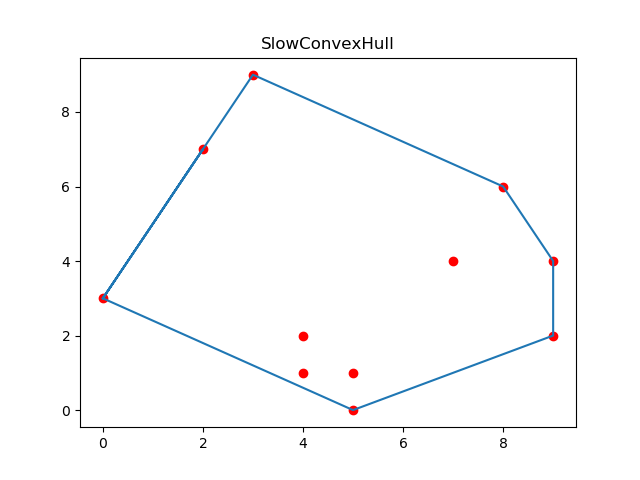
\includegraphics[scale=0.54]{SlowConvexHull}\\
    \tiny{The polygon produced by the SlowConvexHull algorithm from given points marked in red.}
\end{center}

\subsubsection{Generating a list of vertices in clockwise order}

In the lines 2-12 of the algorithm, we have constructed the set of required edges $E$ for $\mathcal{CH}(P)$. From $E$, we want to construct the set $\mathcal{L}$ in line 13 wherein the vertices of $\mathcal{CH}(P)$ are sorted into clockwise order.

The edges in $E$ are directed, so we can easily define the `origin' and `endpoint' of each edge. Because we have selected the edges such that all other points lie to their right, the endpoint of an edge will come after its origin if we are moving along the edges of $\mathcal{CH}(P)$ in a clockwise manner.

\begin{algorithm}[H]
\DontPrintSemicolon 
\KwInput{A set $E$ of directed edges.}
\KwOutput{A list $\mathcal{L}$ containing the vertices sorted in clockwise order.} 
$\mathcal{L} \leftarrow \phi $\;
$\overrightarrow{e} \leftarrow$ an arbitrary edge in $E$\;
Append the origin of $\overrightarrow{e}$ to $\mathcal{L}$.\;
\While{$\vert E \vert > 1$}{
    Remove $\overrightarrow{e}$ from $E$.\;
    $d \leftarrow$ the endpoint of $\overrightarrow{e}$\;
    Append $d$ to $\mathcal{L}$.\;
    $\overrightarrow{e} \leftarrow$ the edge in $E$ whose origin is $d$\;
}
\Return $\mathcal{L}$\;
\caption{\textsc{ClockwiseSorting}($E$)}
\end{algorithm}

When we reach the case where $\vert E \vert = 1$, the endpoint of the remaining edge is necessarily the origin of the very first edge chosen from $E$ in line 2, which is already there in $\mathcal{L}$.

If there are $n$ edges in $E$, then this algorithm is $\mathcal{O}(n^2)$, since we are iterating over $n-1$ edges, and for each edge, we are finding another edge among the remaining edges in line 8 (which takes linear time).

\subsubsection{Running time analysis}

The time analysis for this algorithm is quite simple. When we iterate over all possible pairs $(p,q)$, we are iterating over $n^2 - n$ points (since $p\neq q$). For each of these pairs, we are iterating over the remaining $n-2$ points to check which side of $\overrightarrow{pq}$ they fall on. So the for loop running in lines 2-12 of the algorithm is $\mathcal{O}(n^3)$. We just saw that constructing $\mathcal{L}$ in line 13 is $\mathcal{O}(n^2)$. So, the overall algorithm is $\mathcal{O}(n^3)$.

An algorithm that is cubic in its input size is not at all practical for anything other than the smallest input sizes. We need to be more clever in the design of the algorithm to make it more efficient.

\subsection{Graham's scan}

\subsubsection{The improved algorithm}

We will take a `greedy' approach to develop a more efficient algorithm; that is, at each step, we will add one new vertex to $\mathcal{CH}(P)$, and update the underlying conditions to generate the next new vertex.

When walking along the boundary of a convex polygon in a clockwise manner, it is necessary that we only make `right' turns, not left turns. This is just another way of stating the condition which we had observed previously, that all other vertices of $\mathcal{CH}(P)$ must lie to the right of any of its bounding edges.

In our greedy approach, we will utilise the geometric nature of the problem by taking steps in order of the x-coordinates of the points. If we move from left to right along the upper boundary of a convex polygon, we will only make right turns. So, we can calculate the upper section of the required convex hull using this observation, and similarly compute the lower section of the convex hull by moving from right to left.

Suppose $p_1 \ldots p_{n}$ are the points in $P$ sorted in ascending order of x-coordinate. Consider $\mathcal{L}_{\text{upper}}$ to be the list of vertices forming the upper boundary of the convex hull for $P$. Suppose we have computed $\mathcal{L}_{\text{upper}}$ for $p_1 \ldots p_{i-1}$, and now we want to compute it for $p_1 \ldots p_{i}$. 

We will first append $p_i$ to  $\mathcal{L}_{\text{upper}}$, because $p_i$ being the right-most vertex encountered till now, has to belong to the upper boundary of the convex hull for $p_1 \ldots p_{i}$. Then, if there are more than 2 vertices in $\mathcal{L}_{\text{upper}}$, we will check if the last three vertices present in $\mathcal{L}_{\text{upper}}$ are making a right turn. If yes, we proceed to $p_{i+1}$. If not, we delete the middle vertex among the last three vertices, i.e. the second last vertex, and repeat the right turn check on the new triplet of last three vertices.

The lower boundary of the convex hull, $\mathcal{L}_{\text{lower}}$, can be computed in exactly the same way as $\mathcal{L}_{\text{upper}}$, except that to maintain the right-turn condition, we will move in descending order of x-coordinates.

\begin{algorithm}[H]
\DontPrintSemicolon 
\KwInput{A set $P$ of points in the plane.}
\KwOutput{A list $\mathcal{L}$ containing the vertices of $\mathcal{CH}(P)$ in clockwise order.} 
Sort $P$ by ascending x and then y coordinate, resulting in a sequence $p_1, \ldots, p_n$.\;
$\mathcal{L}_{\text{upper}} \leftarrow \{p_1, p_2\} $\;
\ForEach{$i$ in $3 \ldots n$}{
    Append $p_i$ to $\mathcal{L}_{\text{upper}}$\;
    \While{$ \vert \mathcal{L}_{\text{upper}} \vert > 2$ \textbf{and} the last three points in $\mathcal{L}_{\text{upper}}$ do not make a right turn}{Delete the middle of the last three points from $\mathcal{L}_{\text{upper}}$.\;}
}
$\mathcal{L}_{\text{lower}} \leftarrow \{p_n, p_{n-1}\} $\;
\ForEach{$i$ in $n-2 \ldots 1$}{
    Append $p_i$ to $\mathcal{L}_{\text{lower}}$\;
    \While{$ \vert \mathcal{L}_{\text{lower}} \vert > 2$ \textbf{and} the last three points in $\mathcal{L}_{\text{upper}}$ do not make a right turn}{Delete the middle of the last three points from $\mathcal{L}_{\text{lower}}$.\;}
}
Remove first and last point from $\mathcal{L}_{\text{lower}}$ to avoid duplication of points where lower and upper hull meet.\;
$\mathcal{L} \leftarrow \mathcal{L}_{\text{upper}}$.append( $\mathcal{L}_{\text{lower}}$)\;
\Return $\mathcal{L}$\;
\caption{\textsc{GrahamsScan}($P$)}
\end{algorithm}

$\mathcal{L}_{\text{upper}}$ and $\mathcal{L}_{\text{lower}}$ are concatenated at the end, taking care to remove the repeated leftmost and rightmost points from $\mathcal{L}_{\text{lower}}$, to form the final required list of vertices $\mathcal{L}$. Note that we have accounted for the possibility of two points having the same x-coordinate by sub-sorting on the basis of y-coordinate as well. 

\begin{center}
    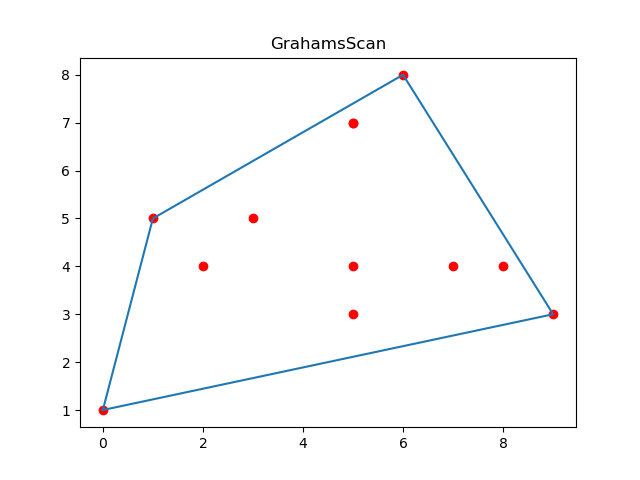
\includegraphics[scale=0.54]{GrahamsScan}\\
    \tiny{The polygon produced by Graham's Scan from given points marked in red.}
\end{center}

\subsubsection{Proving correctness}

We will prove that this algorithm indeed computes the convex hull correctly by induction. The upper hull will be considered first, following which the proof for the lower hull is easily understood.

To prove: For lexicoographically sorted points $p_1, \ldots, p_i$, the upper boundary $\mathcal{L}_{upper}$ computed by Graham's scan lies above all of the points that it does not pass through.

Base case: $i=2$, i.e. the starting point of Graham's scan. The line segment connecting $p_1$ and $p_2$ trivially forms the upper boundary for these two points. 

Induction hypothesis: the claim holds true for $i-1 \in \mathbb{N}$. 

Induction step: to prove that the claim holds true for $i$. By the induction hypothesis, we know that the boundary for $p_1, \ldots, p_{i-1}$ lies on or above all the points in $p_1, \ldots, p_{i-1}$, and it consists entirely of right turns. After adding $p_i$ and running the \textit{while} loop, the updated upper boundary still consists of all right turns and contains both $p_1$ and $p_i$ due to the construction of the algorithm. To guarantee that there is no point above boundary, we only need to check the vertical slab between $p_{i-1}$ and $p_i$, since all the points upto $p_{i-1}$ were already below (or on) the boundary before the addition of $p_i$. But since $p_i$ is the immediate next point to $p_{i-1}$ lexicographically, there can be no point between $p_{i-1}$ and $p_i$. So the boundary for $p_1, \ldots, p_i$ lies on or above all the points in $p_1, \ldots, p_i$. Hence proved. \hfill $\square$

\subsubsection{Running time analysis}

The lexicographic sorting of points in line $1$ can be done in $\mathcal{O}(n\text{log}n)$ time. The \emph{for} loop in lines 3-8 will run $\mathcal{O}(n)$ times. Whenever the while loop in lines 5-7 runs, it deletes one point from the upper (or lower) hull being computed. So cumulatively across all runs of the \emph{for} loop, the \emph{while} loop will run $\mathcal{O}(n)$ time (since there are $\mathcal{O}(n)$ points which can be deleted). Thus, lines 3-8 are overall $\mathcal{O}(n)$, and similarly lines 10-15 are $\mathcal{O}(n)$. The remaining lines take constant time or again $\mathcal{O}(n)$ time in the case of line 17. The overall algorithm is $\mathcal{O}(n\text{log}n)$ only due to the sorting step.

\pagebreak

\section{Line segment intersection}

\subsection{Understanding the problem}

Given two sets of line segments in a plane, we want to compute all points on the plane where any segment from the first set intersects with any segment from the second set. These intersection points will include points where one or both of the segments intersecting have an endpoint at the point of intersection.

To simplify the problem, we can merge the two sets into a single one, and then find all the pairs of segments within this single set which intersect. Once these pairs are found, we just need to select the pairs wherein each segment belonged to a different set originally - this last step is linear in the size of the output, so it is certainly less than or equal to the initial checking of all the possible pairs in terms of time complexity.

The obvious, brute-force method to do this would be to iterate over all possible pairs of segments and check for intersections, resulting in an $\mathcal{O}(n^2)$ algorithm. However, in many cases, the actual number of intersections is much lower than $\mathcal{O}(n^2)$. If we can design an algorithm whose running time is bounded by the number of intersections itself, this will help in increasing the net efficiency.

\subsection{Constructing an algorithm}

\subsubsection{Plane sweeping}

An intuitive way to reduce the number of pairs of segments tested is to consider that segments which are `far apart' cannot intersect. Let us look at how one can formalise this concept of being `far apart'.

Consider the $y$-projection of a line segment, i.e. if the endpoints of the segment are $(x_1,y_1)$ and $(x_2,y_2)$, then its $y$-projection will be the interval $[y_1,y_2]$ on the $y$-axis. If the $y$-projections of two line segments do not intersect, then the segments themselves do not intersect as well - this can easily be seen.

So, only segments who's $y$-projections overlap need to be checked to see if they intersect. How do we know whether two segments fulfil this criteria? We use a sweep line $l$, a horizontal line which moves in a vertical direction - \emph{sweeps} - over the plane containing the segments being tested. In our case, we will take $l$ to move in the vertically downward direction.

Let us define the \emph{status} of $l$ to be the identities of all segments which intersect $l$ at any given time. As $l$ moves downwards over the plane, its status will obviously change. The points at which it changes are (i) the upper endpoints of our line segments, where the status is updated by adding the segment whose upper endpoint has been encountered, and (ii) the lower endpoints, where the status is updated by removing the segment whose lower endpoint was encountered. So, at any given time, we only need to check for intersections between those segments which are part of the status of $l$.

However, this can still end up taking quadratic time in certain cases. Another way to utilise the concept of only testing `close by' segments is to order the segments in the status from left to right. When testing for intersections, we shall only check those pairs of segments which are adjacent to each other in this left-to-right ordering. Obviously, this ordering will change as $l$ moves downwards - the points at which it will change are now not only the endpoints of the segments, but also any intersection points of the segments. So the definition of the \emph{status} is updated to consist of an \emph{ordered} list of all segments which intersect $l$.

\begin{center}
    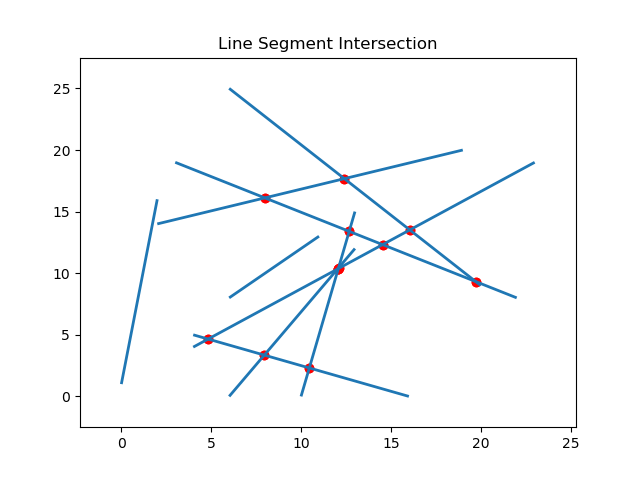
\includegraphics[scale=0.54]{LinSegInt_0}\\
    \tiny{Example 3.1: a result of the Line Segment Intersection algorithm.}
\end{center}

\subsubsection{Ensuring completeness}

Given our approach of only testing adjacent segments along the sweep line $l$ for intersections, we have to confirm that this will actually allow all intersections to be detected. We will ignore some edge cases by making some assumptions that (i) no segment is horizontal and (ii) no more than two segments intersect at any point on the plane. Those points of intersection that occur at the endpoint of a segment will anyway be detected by the sweep line when it reaches that endpoint, since the \emph{status} is checked and updated at endpoints of all segments encountered. So, we need to confirm that our strategy successfully detects the intersections that occur in the interior of the segments.

\textbf{Lemma}. Consider two non-horizontal segments $s_i$ and $s_j$ whose interiors intersect at a point $p$, and there is no third segment that passes through $p$. Then there is some event point above $p$ where $s_i$ and $s_j$ become adjacent and are tested for intersection.

\textbf{Proof}. Suppose $l$ is at a position slightly above $p$, close enough to $p$ such that $s_i$ and $s_j$ are adjacent along $l$ and there is no other event point between the current position of $l$ and $p$. So, there is a position of $l$ where $s_i$ and $s_j$ are adjacent. However, at the very start of the algorithm, when $l$ was at the very top of the plane and not intersecting any segment yet, its status was an empty set, and so $s_i$ and $s_j$ could not have been adjacent along $l$ at that point. Hence, there is some event point encountered between the start and the current position of $l$ wherein $s_i$ and $s_j$ become adjacent and so are tested for intersection.

\subsubsection{Intersection of a pair of segments}

To test whether a single pair of segments $s_i$ and $s_j$ intersect, we shall use a vector-based approach.

Let $s_i$ run from $\mathbf{p}$ to $\mathbf{p+r}$, where $\mathbf{p}$ and $\mathbf{r}$ are vectors. Similarly, let $s_j$ run from $\mathbf{q}$ to $\mathbf{q+s}$. Suppose we extend both segments into lines. Then any point on the first line can be represented by $\mathbf{p} + t\mathbf{r}$, and similarly any point on the second line can be represented by $\mathbf{q} + u\mathbf{s}$, where $t$ and $u$ are scalars.

The two \emph{lines} intersect if $\mathbf{p} + t\mathbf{r}$ = $\mathbf{q} + u\mathbf{s}$ has a solution. Using vector cross-product operations, we can obtain expressions for $t$ and $u$:
\begin{equation*}
    t = (\mathbf{q} - \mathbf{p}) \times \mathbf{s} / (\mathbf{r} \times \mathbf{s}) \hspace{2em} u = (\mathbf{q} - \mathbf{p}) \times \mathbf{r} / (\mathbf{r} \times \mathbf{s})
\end{equation*}

However, such an intersection, if occurs, may also occur at a point not contained within one or both original \emph{segments}. So we need to check different cases to ensure that a correct answer is obtained.

\begin{itemize}
    \item Case 1: If $\mathbf{r} \times \mathbf{s} = 0$ and $(\mathbf{q} - \mathbf{p}) \times \mathbf{r} = 0$, then the two lines are collinear.\\
    In this case, we can express the endpoints of the second segment ($\mathbf{q}$ to $\mathbf{q}+\mathbf{s}$) in terms of the equation of the first line segment ($\mathbf{p} + t\mathbf{r}$):
    \begin{equation*}
        t_0 = (\mathbf{q} - \mathbf{p}) \cdot \mathbf{r} / (\mathbf{r} \cdot \mathbf{r})
    \end{equation*}
    \begin{equation*}
        t_1 = (\mathbf{q} + \mathbf{s} - \mathbf{p}) \cdot \mathbf{r} / (\mathbf{r} \cdot \mathbf{r}) = t_0 + \mathbf{s} \cdot \mathbf{r} / (\mathbf{r} \cdot \mathbf{r})
    \end{equation*}
    If the interval between $t_0$ and $t_1$ intersects the interval [0,1], then the line segments $s_i$ and $s_j$ are collinear and overlapping; otherwise they are collinear and disjoint. \\
    Note that if s and r point in opposite directions, then $\mathbf{s} \cdot \mathbf{r} < 0$, and so the interval to be checked is [$t_1,t_0$] rather than [$t_0,t_1$].
    
    \item Case 2: If $\mathbf{r} \times \mathbf{s} = 0$ and $(\mathbf{q} - \mathbf{p}) \times \mathbf{r} \neq 0$, then the two lines are parallel and non-intersecting.
    
    \item Case 3: If $\mathbf{r} \times \mathbf{s} \neq 0$ and $0 \leq t, u \leq 1$, then the two lines meet at the point $\mathbf{p} + t\mathbf{r} = \mathbf{q} + u\mathbf{s}$.
    
    \item Case 4: Otherwise, the two line segments are not parallel but do not intersect.
\end{itemize}

Running these computations for a single pair of line segments evidently takes constant time.

\subsubsection{Event point handling}

The previously defined `event points' encountered by the sweep line $l$ as it moves downward over the plane can be of three types. For each type, the updates made to the status of $l$ are different.

\begin{enumerate}
    \item The event point is the upper endpoint of a line segment. In this case, $l$ has encountered a previously unseen line segment. This line segment will be tested for intersection with the line segments already present in the status of $l$ which are adjacent to this segment. Only points of intersection below $l$ need to be considered, since the algorithm by construction has already accounted for any points above $l$ at this time. If any such intersection point is found, this is added to the list of event points to be checked. Once this is done, $l$ moves to the next-vertically-closest event point.
    
    \item The event point is the intersection of two line segments (may be in the interior of both line segments or not). In this case, the two intersecting segments will change their order in the left-to-right ordering required by the status of $l$, since the segments are crossing each other. When their order changes, each of these two segments will acquire at most one new neighbour. The algorithm tests for possible intersections with these new neighbours, which, if found, get added to the list of event points to be tested. However, it is possible that an intersection detected in this way may have already been encountered previously if the two segments being tested have been adjacent before. Again, only points of intersection below $l$ need to be taken into consideration.
    
    \item The event point is the lower endpoint of a line segment. In this case, the two neighbours of this line segment will become adjacent, since this segment has `ended'. So these two neighbours will need to be tested for intersection. Note that any intersection point detected in this way may have already been found during a previous step of the algorithm as well.
\end{enumerate}

\subsection{Formalising the method}

\subsubsection{Event queue}

The method we have devised makes extensive use of event points. So we need an efficient way to store, access and modify the event points known at each step of the algorithm.

One initial approach that comes to mind is to use a heap. However, using a heap will not allow us to check whether a certain event is already present in it. Hence, we shall use another type of data structure for this purpose - an event queue ($Q$).

This event queue should be able to implement the following operations:
\begin{itemize}
    \item Identification and removal of the next event point which is to be taken into consideration, so that the algorithm can move to this point for executing the designated steps. This is the event point which is closest to the sweep line $l$ while also remaining vertically below it.
    \item Insertion of new event points which will be identified during computations executed in previous event points. This should incorporate a check of whether the point to be inserted is already present in $Q$.
\end{itemize}

An assumption we have made so far is that all event points have distinct y coordinates. However, this is often not actually the case. In case two or more event points have the same y coordinate, $Q$ will choose the point having the smaller x coordinate to return first.

Another case that we have to take into consideration is that two event points may coincide. For example, two segments may have the same upper endpoint. The ability to check whether a given point is already present in $Q$ will allow us to insert this event point into $Q$ only once, rather than needlessly repeating its insertion and further computations on it.

The balanced binary search tree can be used to efficiently implement this event queue $Q$. The definition of the ordering used by the tree will be as follows: if $p$ and $q$ are two event points, then $p < q$ if and only if ($p_y > q_y$) or ($p_y = q_y$ and $p_x < q_x$).

Each event point stored in $Q$ will be stored along with the segments whose upper endpoint is $p$, which will allow us to easily execute the \textsc{HandleEventPoint} routine described shortly. Using a binary balanced search tree allows both insertion and removal operations to occur in $\mathcal{O}(\text{log} m)$ time, where $m$ is the number of event points in $Q$.

\subsubsection{Status structure}

The status of the sweep line $l$ is another essential part of our method. This consists of the left-to-right ordered list of segments which are intersecting $l$, and it allows us to easily determine the neighbours of any given segment so that they can be tested for intersection with that segment.

Similar to the event queue, the data structure that will be used for this must allow insertions and deletions, while maintaining the defined left-to-right ordering.

Hence, a balanced binary search tree will work well for this requirement too. We will define this tree that stores the status as the status structure $\tau$. The segments currently intersecting $l$ will be stored in the leaves of $tau$, and the ordering used by the tree is the defined left-to-right ordering. At each internal node of $\tau$, the segment present in the rightmost leaf of that segments subtree is stored - this will help the tree efficiently search and access the required segment.  
Suppose the algorithm is currently at some event point $p$ on the sweep line $l$, and we want to find the segment that is immediately adjacent to $p$ on its left. While moving through $\tau$ to find this segment, at each internal node $\nu$, the tree tests whether $P$ lies on the left or the right of the segment stored at $\nu$. Based on the result, the search moves to either the left or right subtree of $\nu$, ending up at a leaf eventually. Either this leaf, or the leaf immediately to its left, will contain the desired segment. The search for a segment immediately to the right of $p$ will occur in a similar fashion.

Again, due to using the binary search tree, each insertion and search operation will take $\mathcal{O}(\text{log}(n))$ time.

\subsubsection{The algorithm}

\begin{algorithm}[H]
\DontPrintSemicolon 
\KwInput{A set $S$ of line segments in the plane.}
\KwOutput{The set of intersection points among the segments in $S$, along with the segments that contain each intersection point.}
Initialize an empty event queue $Q$.\;
Insert the segment endpoints into $Q$. When an upper endpoint is inserted, the corresponding segment should be stored with it.\;
Initialize an empty status structure $\tau$.\;
\While{$Q$ \text{is not empty}}{Determine the next event point $p$ in $Q$ and delete it.\; \textsc{HandleEventPoint}$(p)$\;}
\caption{\textsc{FindIntersections}($S$)}
\end{algorithm}

\begin{algorithm}[H]
\DontPrintSemicolon 
Let $U(p)$ be the set of segments whose upper endpoints is $p$; these segments are stored with the event point $p$. For horizontal segments, the upper endpoint is by definition the left endpoint.\;
Find all segments stored in $\tau$ that contain $p$; they are adjacent in $\tau$.\;
Let $L(p)$ denote the subset of segments found whose lower endpoint is $p$, and let $C(p)$ denote the subset of segments found that contain $p$ in their interior.\;
\If{$L(p) \cup U(p) \cup C(p)$ \text{contains more than one segment}}{Report $p$ as an intersection, together with $L(p), U(p)$ and $C(p)$.\;}
Delete the segments in $L(p) \cup C(p)$ from $\tau$.\;
Insert the segments in $U(p) \cup C(p)$ into $\tau$. The order of the segments in $\tau$ should correspond to the order in which they are intersected by a sweep line just below $p$. If there is a horizontal segment, it comes last among all segments containing $p$.\;
\If{$U(p) \cup C(p) = \phi$}{Let $s_l$ and $s_r$ be the left and right neighbours of $p$ in $\tau$.\; \textsc{FindNewEvent}$(s_l,s_r,p)$\;}
\Else{
Let $s'$ be the leftmost segment of $U(p) \cup C(p)$ in $\tau$.\;
Let $s_l$ be the left neighbour of $s'$ in $\tau$.\;
\textsc{FindNewEvent}$(s_l,s',p)$\;}
\caption{\textsc{HandleEventPoint}$(p)$
Let $s"$ be the rightmost segment of $U(p) \cup C(p)$ in $\tau$.\;
Let $s_r$ be the left neighbour of $s"$ in $\tau$.\;
\textsc{FindNewEvent}$(s",s_r,p)$\;}
\caption{\textsc{HandleEventPoint}$(p)$
}
\end{algorithm}

\begin{algorithm}[H]
\DontPrintSemicolon 
\If{$s_l$ \text{and} $s_r$ \text{intersect below the sweep line, or on it and to the right of the current event point} $p$\text{, and the intersection is not yet present as an event in $Q$}}{Insert the intersection point as an event into $Q$.\;}
\caption{\textsc{FindNewEvent}$(s_l,s_r,p)$}
\end{algorithm}

\subsubsection{Proving correctness}

\textbf{Lemma}. Our algorithm correctly identifies all intersection points and the segments that contain them.

\textbf{Proof}. The priority of the ordering used by $Q$ as defined is that if $p$ and $q$ are two event points, then $p < q$ if and only if ($p_y > q_y$) or ($p_y = q_y$ and $p_x < q_x$). The lemma can be proved by induction on these priorities of the event points.

Let $p$ be an intersection point of two segments. By the induction hypothesis, we can assume that all intersection points $q$ with a higher priority than $p$ have been computed correctly. We shall prove that $p$ and the segments that contain $p$ are computed correctly. Let $U(p)$ be the set of segments that have $p$ as their upper endpoint, let $L(p)$ be the set of segments having p as their lower endpoint, and let $C(p)$ be the set of segments having $p$ in their interior.

\begin{center}
    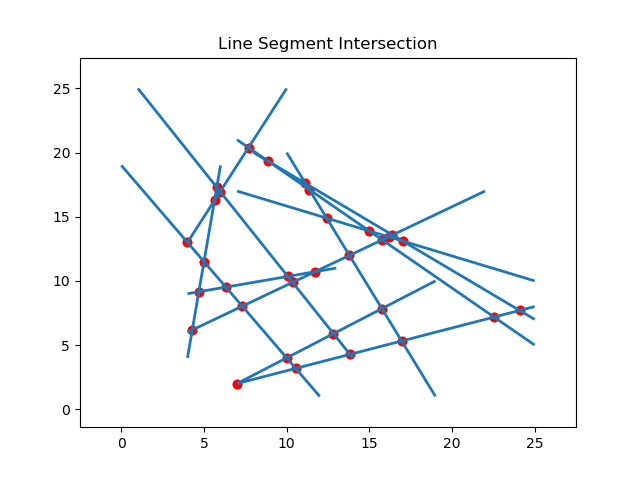
\includegraphics[scale=0.54]{LinSegInt_1}\\
    \tiny{Example 3.2: a result of the Line Segment Intersection algorithm.}
\end{center}

First, let us consider the case where $p$ is an endpoint of one or more of the segments. Here, $p$ will be stored in the event queue at the start of the algorithm. The segments from $U(p)$ are stored with $p$, so they will easily be found from $Q$. The segments from $L(p)$ and $C(p)$ are stored in $\tau$ when $p$ is handled, so they will be found in line 2 of the \textsc{HandleEventPoint} subroutine. Hence, $p$ and all the segments involved are determined correctly in this case.

Now consider the case where $p$ is not an endpoint of a segment. We need to show that $p$ will be inserted into $Q$ at some moment. All segments that are involved will have $p$ in their interior. We can order these segments by angle around $p$. Let $s_i$ and $s_j$ be two neighboring segments in the resulting order. From our previous lemma, we know that there is an event point $q$ with a higher priority than $p$ such that $s_i$ and $s_j$ become adjacent when $q$ is passed. By induction, the event point $q$ was handled correctly, which means that $p$ is detected and stored into $Q$. \hfill $\blacksquare$


\end{document}
